% The contents of this file is 
% Copyright (c) 2021-  David S. Read and Dr. Christine Reilly, All Rights Reserved


% LATEXONLY

\sloppy
%\setlength{\topmargin}{-0.375in}
%\setlength{\oddsidemargin}{0.0in}
%\setlength{\evensidemargin}{0.0in}

% Uncomment these to center on 8.5 x 11
%\setlength{\topmargin}{0.625in}
%\setlength{\oddsidemargin}{0.875in}
%\setlength{\evensidemargin}{0.875in}

%\setlength{\textheight}{7.2in}

\setlength{\headsep}{3ex}
\setlength{\parindent}{0.0in}
\setlength{\parskip}{1.7ex plus 0.5ex minus 0.5ex}
\renewcommand{\baselinestretch}{1.02}

% see LaTeX Companion page 62
\setlength{\topsep}{-0.0\parskip}
\setlength{\partopsep}{-0.5\parskip}
\setlength{\itemindent}{0.0in}
\setlength{\listparindent}{0.0in}

% see LaTeX Companion page 26
% these are copied from /usr/local/teTeX/share/texmf/tex/latex/base/book.cls
% all I changed is afterskip

\makeatletter

\renewcommand{\section}{\@startsection 
    {section} {1} {0mm}%
    {-3.5ex \@plus -1ex \@minus -.2ex}%
    {0.7ex \@plus.2ex}%
    {\normalfont\Large\bfseries}}
\renewcommand\subsection{\@startsection {subsection}{2}{0mm}%
    {-3.25ex\@plus -1ex \@minus -.2ex}%
    {0.3ex \@plus .2ex}%
    {\normalfont\large\bfseries}}
\renewcommand\subsubsection{\@startsection {subsubsection}{3}{0mm}%
    {-3.25ex\@plus -1ex \@minus -.2ex}%
    {0.3ex \@plus .2ex}%
    {\normalfont\normalsize\bfseries}}

% The following line adds a little extra space to the column
% in which the Section numbers appear in the table of contents
\renewcommand{\l@section}{\@dottedtocline{1}{1.5em}{3.0em}}
\setcounter{tocdepth}{1}

\makeatother

\newcommand{\beforefig}{\vspace{1.3\parskip}}
\newcommand{\afterfig}{\vspace{-0.2\parskip}}

\newcommand{\beforeverb}{\vspace{0.6\parskip\fontsize{9}{11}}}
\newcommand{\afterverb}{\vspace{0.6\parskip\normalsize}}

\newcommand{\adjustpage}[1]{\enlargethispage{#1\baselineskip}}


% Note: the following command seems to cause problems for Acroreader
% on Windows, so for now I am overriding it.
%\newcommand{\clearemptydoublepage}{
%            \newpage{\pagestyle{empty}\cleardoublepage}}
\newcommand{\clearemptydoublepage}{\cleardoublepage}

%\newcommand{\blankpage}{\pagestyle{empty}\vspace*{1in}\newpage}
\newcommand{\blankpage}{\vspace*{1in}\newpage}

% HEADERS

\renewcommand{\chaptermark}[1]{\markboth{#1}{}}
\renewcommand{\sectionmark}[1]{\markright{\thesection\ #1}{}}

\lhead[\fancyplain{}{\bfseries\thepage}]%
      {\fancyplain{}{\bfseries\rightmark}}
\rhead[\fancyplain{}{\bfseries\leftmark}]%
      {\fancyplain{}{\bfseries\thepage}}
\cfoot{}

\pagestyle{fancyplain}


% turn off the rule under the header
%\setlength{\headrulewidth}{0pt}

% the following is a brute-force way to prevent the headers
% from getting transformed into all-caps
\renewcommand\MakeUppercase{}

% Exercise environment
\newtheoremstyle{myex}% name
     {9pt}%      Space above
     {9pt}%      Space below
     {}%         Body font
     {}%         Indent amount (empty = no indent, \parindent = para indent)
     {\bfseries}% Thm head font
     {}%        Punctuation after thm head
     {0.5em}%     Space after thm head: " " = normal interword space;
           %       \newline = linebreak
     {}%         Thm head spec (can be left empty, meaning `normal')

\theoremstyle{myex}


\newtheorem{ex}{Exercise}[chapter]

\begin{latexonly}

\renewcommand{\blankpage}{\thispagestyle{empty} \quad \newpage}

\thispagestyle{empty}

%\begin{flushright}
%\vspace*{2.0in}

%\begin{spacing}{3}
%{\huge Introduction to Computer Science and Programming}\\
%{\Large Python Edition}
%\end{spacing}

%\vspace{0.25in}

%Version \theversion

%\vspace{0.5in}


%{\Large
%David Read\\
%}

%\vfill

%\end{flushright}

\begin{titlepage}
%	\centering
		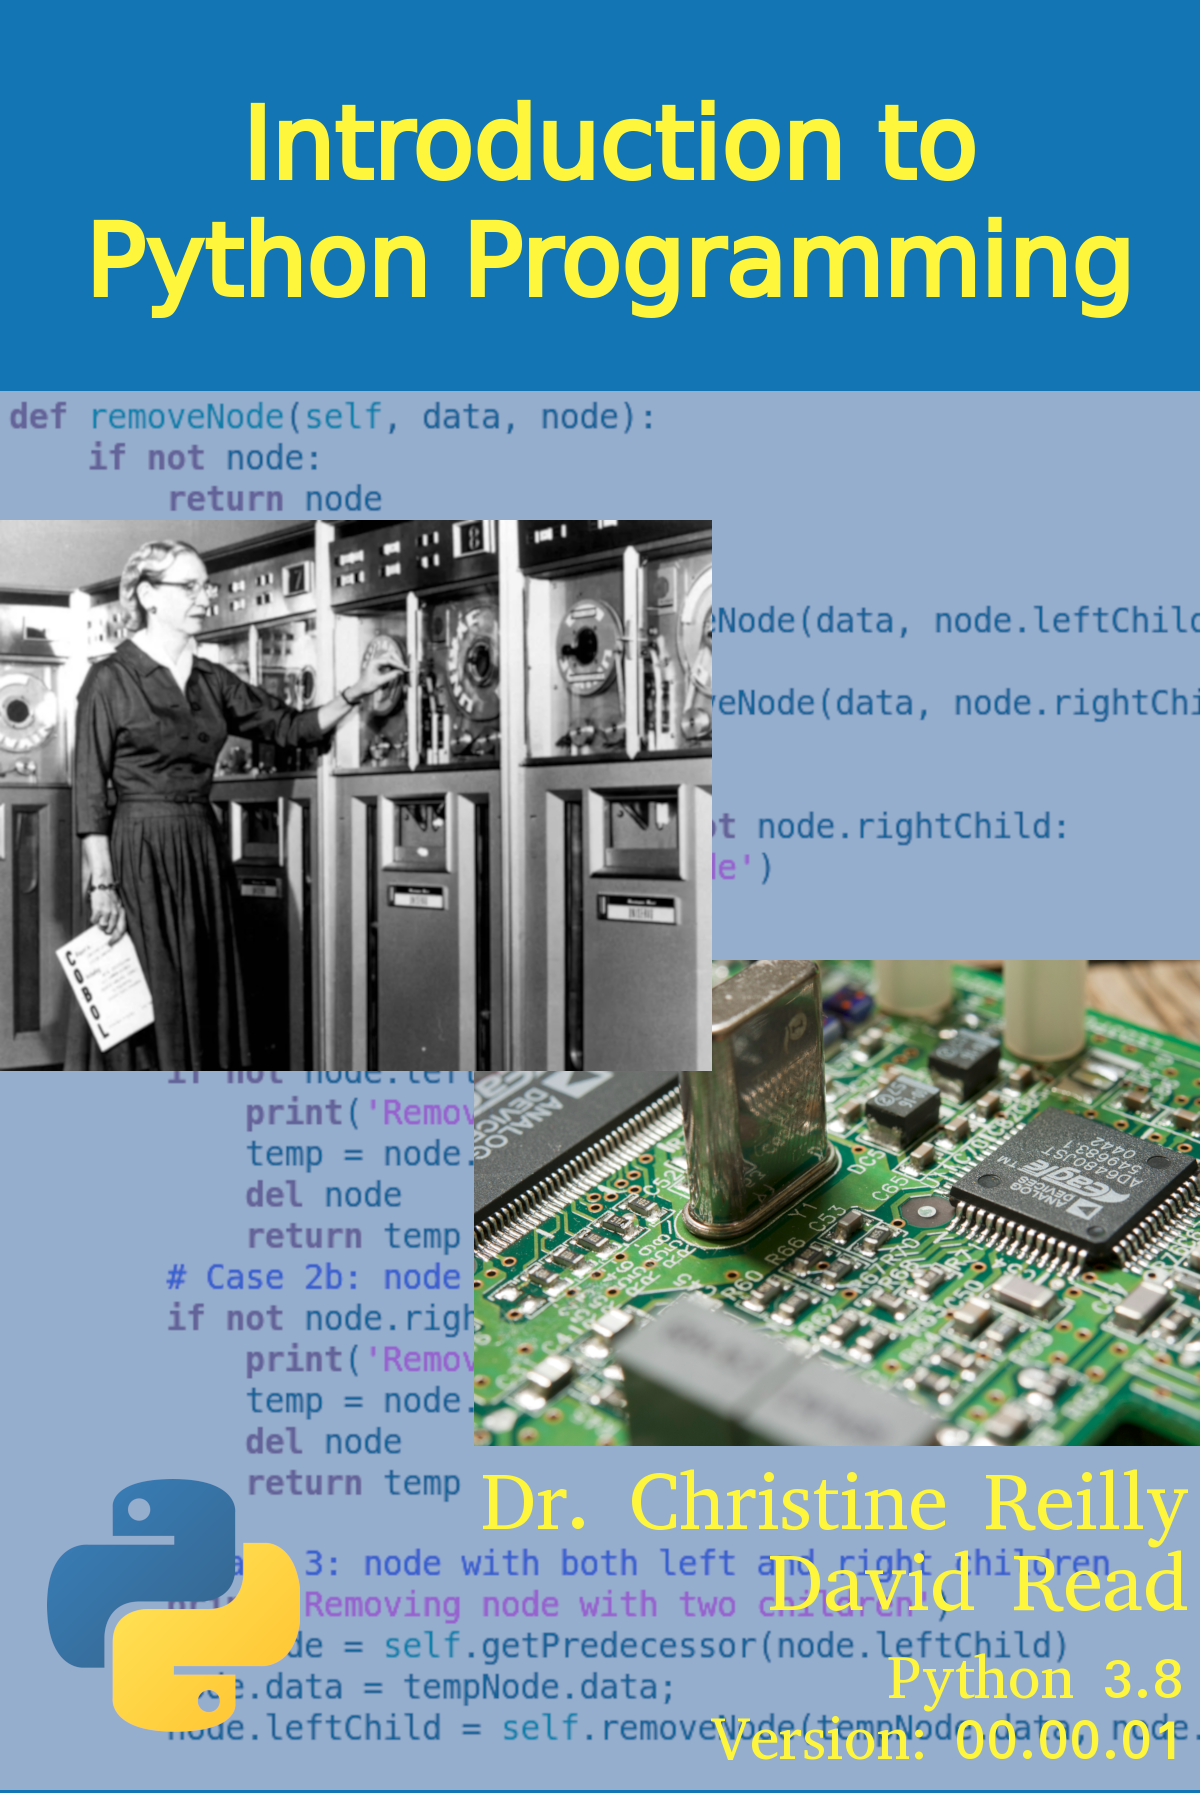
\includegraphics[width=5.25in]{python-cover/CoverBackground.png}
\end{titlepage}

%--copyright--------------------------------------------------
\pagebreak
\thispagestyle{empty}

{\small
Copyright \copyright ~2021- David S. Read and Dr. Christine Reilly

\underline{\textbf{Cover art:}}

Navy admiral Grace Hopper. Creative Commons Attribution
\newline
\url{https://tophat.com/blog/grace-hopper-yale-computer-science/}

Circuit board. Creative Commons Zero license
\newline \url{https://www.needpix.com/photo/download/1800090/pcb-printed-circuit-board-components-electronic-resistor-transistor-capacitor}

Python Logo. www.python.org, GPL via Wikimedia Commons
\newline
\url{http://www.gnu.org/licenses/gpl.html} 



\underline{\textbf{Printing history:}}

\begin{description}
	
\item[June 2021:] Added sample text from the mbox-small.txt file to chapters 9 (lists) and 12 (regular expressions) to clarify the output dsplayed by the sample code. Thank you to students Emily Hey and Sloane Zwanger for suggesting this update.

\item[May 2021:] Fixed minor errata found during the spring 2021 semester. Updated string formatting to use more recent \{\} syntax (See: \url{https://docs.python.org/3/library/string.html\#string.Formatter})

\item[January 2021:] Using chapters 1-16 of \emph{Python for Informatics: Exploring Information} and material from chapters 1-8 of \emph{Introduction to Computer Science and Programming, Java Edition} to create a textbook for a 100-level Python introductory course.

\item[July 2019:] Cleanup of Methods chapter, including moving OO instances discussion into a separate appendix.

\item[January 2019:] Minor clarifications and cleanup throughout the chapters.

\item[July 2018:] Minor text cleanup in chapter 1 (variables). Clarified the exercise description in chapter 6. Modified Pi Lab 7 to simplify the wiring (reducing from 8 LEDs to 5).

\item[December 2017:] Minor text updates in chapter 6 (Strings) including moving scattered exercises to the end of the chapter. Updated debugging instructions for PiLab operation in Appendix B (Pi Labs)
	
\item[October 2017:] Fixed definite and indefinite loops discussion regarding while and for statements in chapter 5 (iteration)

\item[August 2017:] Added section on casting to chapter 1 and updated Raspberry Pi setup instructions based on raspi-config changes
	
\item[December 2016:] Minor typographical updates

\item[September 2016:] Example code cleanup

\item[August 2016:] Updated and extended the Pi setup documentation

\item[June 2016:] Added content specific to Raspberry Pi (appendices for Pi setup and labs)

\item[May 2016:] General cleanup and editing

\item[April 2016:] Added a new chapter on recursion (chapter 7). Major revisions to chapter 8.

\item[March 2016:] Major revisions to chapter 6

\item[February 2016:] Major revisions to chapters 4 and 5

\item[January 2016:] Major revisions to chapters 0 through 3 beginning the creation of a Java textbook \emph{Introduction to Computer Science and Programming, Java Edition} from \emph{Python for Informatics: Exploring Information} by \emph{Dr. Charles R. Severance}.

\item[December 2015:] Editorial pass thanks to Sue Blumenberg.

\item[October 2013:] Major revision to Chapters 13 and 14
to switch to JSON and use OAuth.
Added new chapter on Visualization.

\item[September 2013:] Published book on Amazon CreateSpace

\item[January 2010:] Published book using the University of 
Michigan Espresso Book machine.

\item[December 2009:] Major revision to chapters 2-10 from
\emph{Think Python: How to Think Like
a Computer Scientist}
and writing chapters 1 and 11-15 to
produce 
\emph{Python for Informatics: Exploring Information}

\item[June 2008:] Major revision, changed title to
\emph{Think Python: How to Think Like
a Computer Scientist}.

\item[August 2007:] Major revision, changed title to
\emph{How to Think Like a (Python) Programmer}.

\item[April 2002:] First edition of \emph{How to Think Like
a Computer Scientist}.

\end{description}

\vspace{0.2in}

This work is licensed under a 
Creative Common
Attribution-NonCommercial-ShareAlike 3.0 Unported License.
This license is 
available at
\url{http://creativecommons.org/licenses/by-nc-sa/3.0/}.  You can 
see what the author considers commercial and non-commercial
uses of this material as well as license exemptions 
in the Appendix titled Copyright Detail.

The \LaTeX\ source for the 
\emph{Think Python: How to Think Like
a Computer Scientist}
version of this book is available from
\url{http://www.thinkpython.com}.

\vspace{0.2in}

} % end small

\end{latexonly}


% HTMLONLY

%\begin{htmlonly}

% TITLE PAGE FOR HTML VERSION

{\Large \thetitle}

{\large David Read and Dr. Christine Reilly}

Version \theversion

\setcounter{chapter}{0}

%\end{htmlonly}
